\documentclass[12pt]{article}
\usepackage[top=1in,left=1in, right = 1in, footskip=1in]{geometry}

\usepackage{graphicx}
%\usepackage{adjustbox}

\newcommand{\eref}[1]{(\ref{eq:#1})}
\newcommand{\fref}[1]{Fig.~\ref{fig:#1}}
\newcommand{\Fref}[1]{Fig.~\ref{fig:#1}}
\newcommand{\sref}[1]{Sec.~\ref{#1}}
\newcommand{\frange}[2]{Fig.~\ref{fig:#1}--\ref{fig:#2}}
\newcommand{\tref}[1]{Table~\ref{tab:#1}}
\newcommand{\tlab}[1]{\label{tab:#1}}
\newcommand{\seminar}{SE\mbox{$^m$}I\mbox{$^n$}R}

\usepackage{amsthm}
\usepackage{amsmath}
\usepackage{amssymb}
\usepackage{amsfonts}

% \usepackage{lineno}
% \linenumbers

\usepackage[pdfencoding=auto, psdextra]{hyperref}

\usepackage{natbib}
\bibliographystyle{chicago}
\date{\today}

\usepackage{xspace}
\newcommand*{\ie}{i.e.\@\xspace}

\usepackage{color}

\newcommand{\Rx}[1]{\ensuremath{{\mathcal R}_{#1}}} 
\newcommand{\Ro}{\Rx{0}}
\newcommand{\RR}{\ensuremath{{\mathcal R}}}
\newcommand{\Rhat}{\ensuremath{{\hat\RR}}}
\newcommand{\tsub}[2]{#1_{{\textrm{\tiny #2}}}}

\newcommand{\comment}[3]{\textcolor{#1}{\textbf{[#2: }\textsl{#3}\textbf{]}}}
\newcommand{\jd}[1]{\comment{cyan}{JD}{#1}}
\newcommand{\swp}[1]{\comment{magenta}{SWP}{#1}}

\begin{document}

\begin{flushleft}{
	\Large
	\textbf\newline{
		Biases in early-outbreak estimates of epidemiological delay distributions: applications to COVID-19 outbreak
	}
}
\end{flushleft}

\section*{Abstract}

\pagebreak

\section{Introduction}

In December 2019, a cluster of pneumonia cases of unknown etiology was reported in China.
The disease, now referred to as the coronavirus disease 2019 (COVID-19), has since affected more than ??? countries.
As of XXX, more than XXX deaths have been confirmed.

\swp{Skipping introduction for now.}

\jd{This part of intro can be short; we no longer really need to remind people what COVID19 is.}

Understanding the time delays between key epidemiological events, is a key component of statistical and modeling efforts to predict and control disease outbreaks. 
These events can be compared within an infected individual (e.g., the incubaton period is the time between infection and symptom onset) or between infected individuals (e.g., the serial interval is the time between symptom onsets of an infector and an infectee).
However, the estimation of these epidemiological delay distributions depends on having observed both events;
this dependency can bias the estimates during an early growth phase of an outbreak.

\section{Theoretical framework}

We begin by modeling epidemiological delays from a cohort perspective.
A ``cohort'' consists of all individuals whose first epidemiological event of interest occurred at a given time.
For example, for the purpose of measuring the symptomatic period, cohort $s$ consists of all individuals who became symptomatic at time $s$.

\jd{Is it going to be better to define a cohort for every epidemiological event, rather than just the ones that \emph{start} an interval? I'm thinking of how useful backwards GIs have been.}
\jd{On the other hand, I like some of the simplicities below.}

Observed delay distributions are generally subject to right-censoring.
Since events must occur before the time of measurement to be observed, delays in cohort $s$ that are longer than $t-s$ cannot be observed at time $t$.
Therefore, the cohort delay distribution $c_s(\tau|t)$ can be expressed as a truncated distribution:
\begin{equation}
c_s(\tau|t) = \frac{f_s(\tau)}{F_s(t-s)},\quad \tau \leq t-s
\end{equation}
where $f_s(\tau)$ is the true delay distribution (which can vary across cohorts) and $F_s(\tau)$ is the corresponding cumulative distribution function.

Other biases also need to be accounted for. Delay distributions involving more than one individual typically change with disease dynamics. For example, serial intervals will be shorter when the number of susceptibles is decreasing rapidly, since there will be fewer infection opportunities as the cohort grows older.
Within-individual delay distributions that depend on external factors (e.g., time between symptom onset and hospitalization) can also change over time.

\begin{figure}[!th]
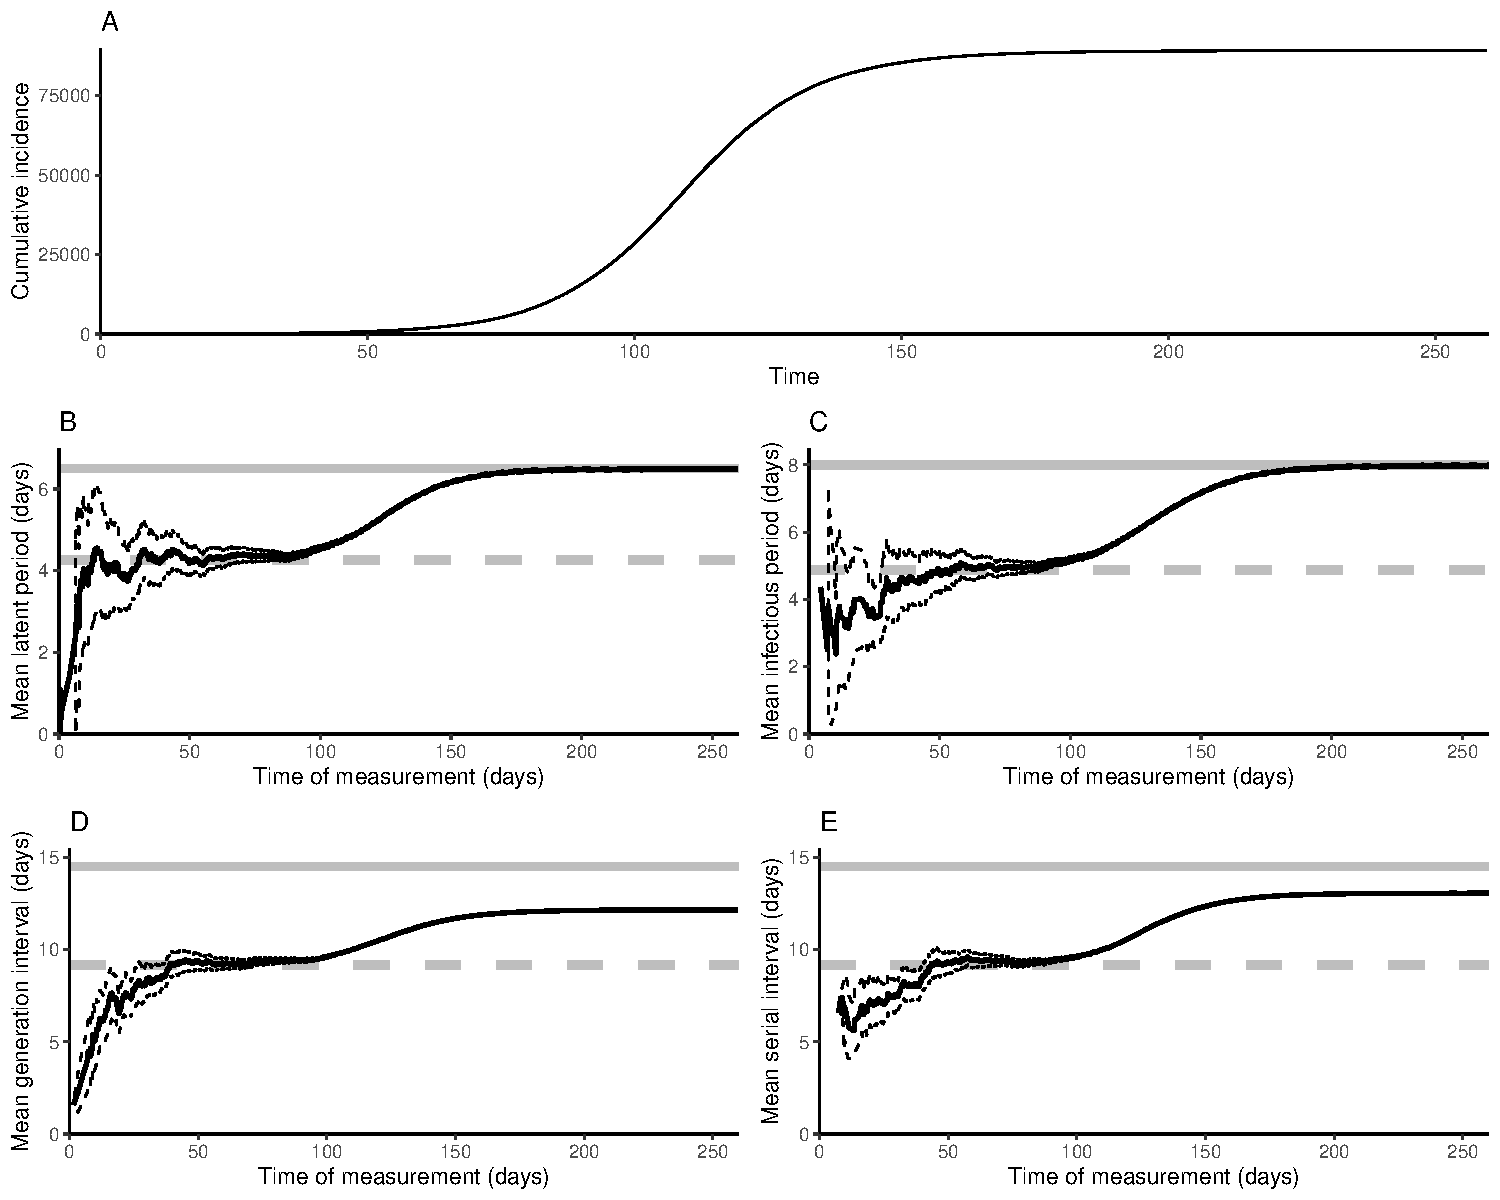
\includegraphics[width=\textwidth]{figure_seir.pdf}
\caption{
\textbf{Observed means of epidemiological delay distributions over time.}
Changes in the observed mean latent period (A), infectious period (B), generation interval (C), and serial interval (D) over the course of an epidemic.
Black solid lines represent the observed mean and associated 95\% confidence intervals at each time of measurement.
Gray solid lines represent the theoretical true mean.
Gray dashed lines represent the theoretical observed mean during the exponential growth phase (calculated via \eref{exp}).
A stochastic SEIR model was simulated using a COVID-like parameters: $\mathcal R_0 = 2.5$, $1/\sigma = 6.5\,\textrm{days}$, $1/\gamma = 8\,\textrm{days}$, $N=100000$, and $I(0)=10$.
}
\label{fig:seir}
\end{figure}

Typically, epidemiological delay distributions are estimated by using all available samples.
Then, the observed delay distribution $f_{\tiny\textrm{obs}}(\tau|t)$, which takes into account all measured delays until time $t$, is equivalent to the average of the cohort delay distributions $c_s(\tau|t)$, weighted by the size of cohorts $i(s)$ and the probability that both epidemiological events of interest will occur between time $s$ and $t$:
\begin{equation}
\begin{aligned}
f_{\tiny\textrm{obs}}(\tau|t) &\propto \int_{-\infty}^{t-\tau} c_s(\tau|t) i(s) F_s(t-s) ds\\
&= \int_{-\infty}^{t-\tau} i(s) f_s(\tau) ds
\end{aligned}
\end{equation}

Early in an epidemic, the incidence of infection, and therefore the size of cohorts, is expected to grow exponentially: $i(s) = i(0) \exp(rs)$.
If we assume that the true delay distribution stays constant for both within- and between-individual delays during this period: $f_s(\tau) = f(\tau)$.
Then, the observed delay distribution during the exponential growth phase $f_{\tiny\textrm{exp}}(\tau|t)$ is equivalent to the true distribution deweighted by the exponential growth rate:
\begin{equation}
\begin{aligned}
f_{\tiny\textrm{exp}}(\tau|t) &\propto f(\tau) \int_{-\infty}^{t-\tau} \exp(rs) ds\\
&\propto f(\tau) \exp(-r\tau) \\
\end{aligned}
\end{equation}
In other words, for fast-growing epidemics (high $r$), there will be a stronger bias to observe shorter intervals.
This bias applies to all epidemiological delay distributions.

\begin{figure}[!th]
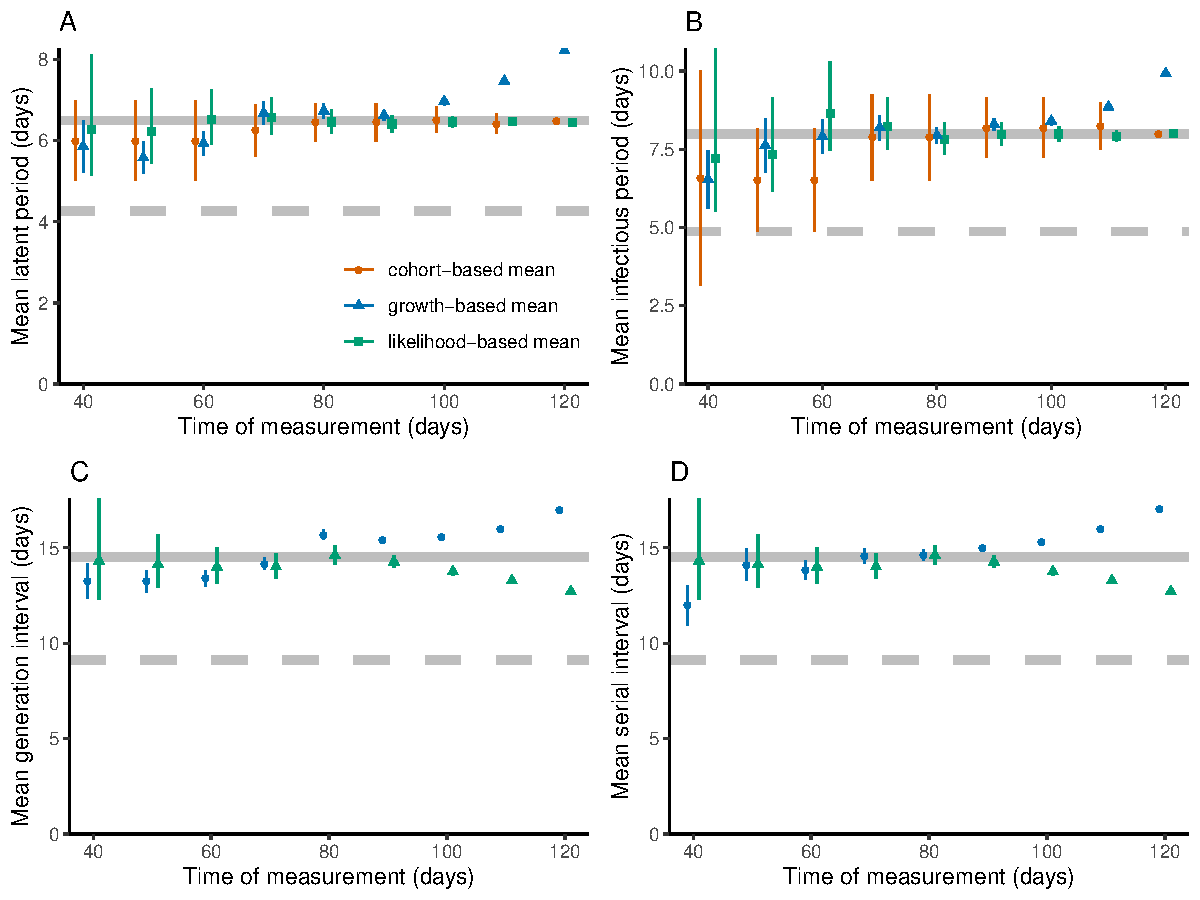
\includegraphics[width=\textwidth]{figure_seir2.pdf}
\caption{
\textbf{Estimated means of epidemiological delay distributions over time.}
Changes in the estimated mean latent period (A), infectious period (B), generation interval (C), and serial interval (D) over the course of an epidemic.
Black solid lines represent the estimated mean and associated 95\% confidence intervals at each time of measurement using the exponential adjustment.
Red solid lines represent the estimated mean and associated 95\% confidence intervals at each time of measurement using the cohort-based adjustment.
Gray solid lines represent the theoretical true mean.
Gray dashed lines represent the theoretical observed mean during the exponential growth phase (calculated via \eref{exp}).
A stochastic SEIR model was simulated using the following parameters: $\mathcal R_0 = 2.5$, $1/\sigma = 6.5\,\textrm{days}$, $1/\gamma = 8\,\textrm{days}$, $N=50000$, and $I(0)=10$.
}
\label{fig:seir2}
\end{figure}

We compare how the observed mean latent period, infectious period, generation interval, and serial interval (assuming that the latent period is equivalent to the incubation period) change over time using an individual-based stochastic simulation of the SEIR model (\fref{seir}).
The stochastic simulation confirms the bias: the observed mean delay during the exponential growth phase matches the theoretical mean that we calculate using \eref{exp}.
The amount of bias decreases as the epidemic progresses;
eventually, the observed mean latent and infectious periods become unbiased.
On the other hand, mean mean observed generation and serial intervals remain biased even at the end of an epidemic because the depletion of the susceptible pool over time makes the realized generation intervals shorter over time.
The serial interval has a slightly higher observed mean than the generation interval near the end of an epidemic because an infected individual with a short latent period (and hence shorter incubation period) is more likely infect others by having a shorter generation interval during the susceptible depletion phase; therefore, infectors are more likely to have shorter latent periods than their infectees.

Equation~\eref{exp} suggests a straightforward way of correcting the bias -- by weighting the observed distribution by the exponential growth rate:
\begin{equation}
\label{eq:exp}
f(\tau) = f_{\tiny\textrm{exp}}(\tau|t) \exp(r \tau).
\end{equation}
Similar forms have been suggested by other studies and applied in estimating epidemiological delay distributions;
however, our simulations show that this naive approach does not work very well for estimating the mean (\fref{seir2}; exponential adjustment).
Although the estimated mean delay is similar to the true mean, the estimates are sensitive, and their associated confidence intervals are narrow.
Once the exponential growth phase is over, applying the exponential adjustment overestimates the mean delay.

Alternatively, we can account for the bias by ensuring that the right-censoring does not exist:
instead of using all samples that have been collected until the time of measurement, we can limit our samples to cohorts within which all individuals have completed both epidemiological events of interest.
This approach gives an unbiased estimate of the mean delay throughout the epidemic with appropriately wide confidence intervals that contain the true value (\fref{seir2}; cohort-based adjustment).
Conversely, the proportion of individuals that have not completed the second event within each cohort is indicative of the amount of bias present in the estimate.
This approach cannot be applied to generation or serial intervals because we don't know how many individuals each person infected (i.e., we cannot measure the degree of right-censoring).
Nonetheless, likelihood-based methods that explicitly account for the right-censoring can be still applied to estimate the generation interval distribution.

\section{Applications: incubation period distribution of COVID-19}

Here, we revisit the incubation period distribution estimated by \cite{backer2020incubation} and assess the degree of bias in their estimate.
Since they relied on early traveler data who traveled from Wuhan between January 2--23, during which the epidemic was likely to have been expanding exponentially, we can expect the number of infected travelers from Wuhan to increase exponentially.
Therefore, their estimate of the mean \emph{observed} incubation periods of 6.4 days (95\% CI: 5.6–7.7 days) is likely to have been subject to right-censoring that we described earlier.

\begin{figure}[!th]
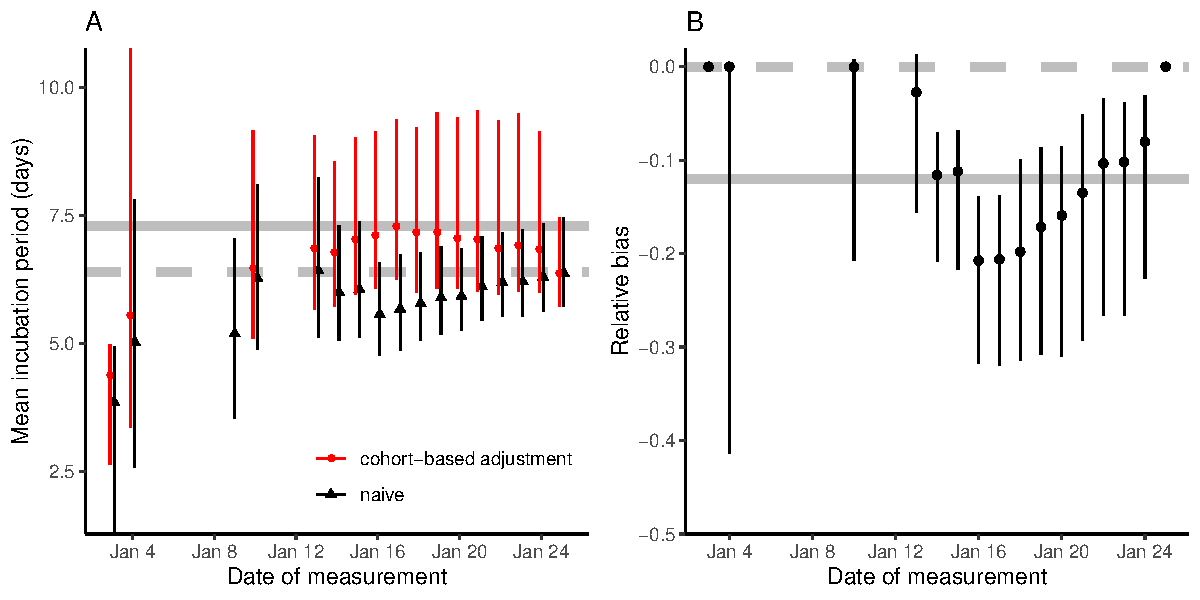
\includegraphics[width=\textwidth]{figure_baker.pdf}
\caption{
\textbf{caption.}
caption
}
\label{fig:baker}
\end{figure}

\fref{fig:baker}A compares the naive mean, which uses all available measurements, with the cohort-based adjusted mean (see Methods for details).
Consistent with out simulations, the cohort-based adjusted mean generally has a higher median and wider confidence intervals (see January 13--24 in \fref{fig:baker}A).
The medians of the cohort-based adjusted means also match the exponentially adjusted mean.
On January 25, two estimates completely overlap because they both use all available samples.
Since \fref{fig:baker}A compares the marginal posterior distributions of the means, it does not allow us to assess whether the cohort-based adjusted mean is higher than the naive mean -- the overlapping confidence intervals do not imply that the differences are not clear.

\fref{fig:baker}B compares the relative bias of the 

% For example, if the observed incubation period follows a gamma distribution with mean of 6.5 days with standard deviation of 2.6 days \citep{backer2020incubation} and the epidemic grows exponentially at rate 1 per week, the true incubation period will have a mean 7.6 days.

\section{Discussion}



\section{Materials and Methods}

\subsection{Stochastic simulations}

See Park, Champredon, and Dushoff (2019) in bioRxiv.

\bibliography{censor}

\end{document}
